\documentclass{article}
\usepackage{amsmath}
\usepackage{amssymb}
\usepackage{microtype}
\usepackage{graphicx}
\usepackage{subfigure}
\usepackage{booktabs} % for professional tables


\usepackage{hyperref}
\usepackage{array}

% Attempt to make hyperref and algorithmic work together better:
\newcommand{\theHalgorithm}{\arabic{algorithm}}

\usepackage[accepted]{icml2021}

% The \icmltitle you define below is probably too long as a header.
% Therefore, a short form for the running title is supplied here:
\icmltitlerunning{Image Animation with Keypoint Mask}

\begin{document}

\twocolumn[
\icmltitle{Image Animation with Keypoint Mask}

\icmlsetsymbol{equal}{*}

\begin{icmlauthorlist}
\icmlauthor{Or Toledano}{tlv}
\icmlauthor{Yanir Marmor}{tlv}
\icmlauthor{Dov Gertz}{tlv}

\end{icmlauthorlist}

\icmlaffiliation{tlv}{Tel Aviv University}

\icmlcorrespondingauthor{Or Toledano}{ortoledano@protonmail.com}
\icmlcorrespondingauthor{Yanir Marmor}{yanirmr@gmail.com}
\icmlcorrespondingauthor{Dov Gertz}{dovgertz1@gmail.com}


\icmlkeywords{Machine Learning, ICML}

\vskip 0.3in
]
\printAffiliationsAndNotice{}

\begin{table}[t]
\caption{\textbf{Motion transfer example:} Given a YouTube clip of a
Thai-Chi artist (top), and an image of another one, our method
transfers the one’s performance onto the other (bottom).}
\label{table:intro}
\vskip 0.15in
\begin{center}
\begin{small}
\begin{sc}
\begin{tabular}{m{1.0cm}m{1.0cm}m{1.0cm}m{1.0cm}m{1.0cm}m{1.0cm}}
\toprule
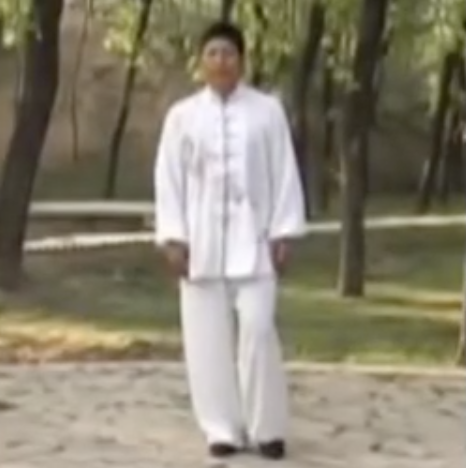
\includegraphics[width=1cm, height=1cm]{images/intro_image/Driving_1.png} &
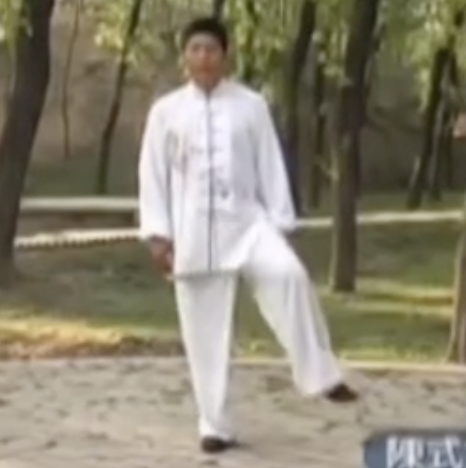
\includegraphics[width=1cm, height=1cm]{images/intro_image/Driving_2.png} &
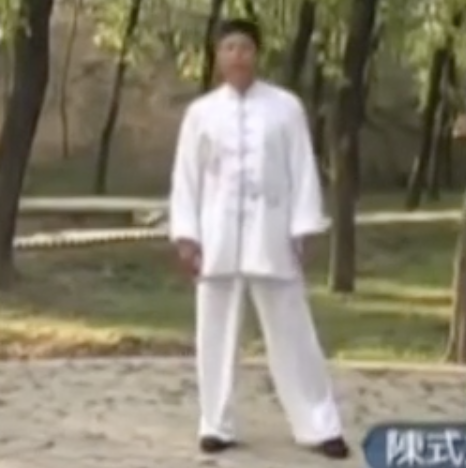
\includegraphics[width=1cm, height=1cm]{images/intro_image/Driving_3.png} &
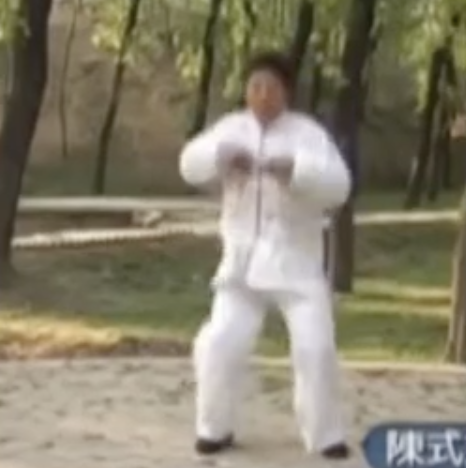
\includegraphics[width=1cm, height=1cm]{images/intro_image/Driving_4.png} &
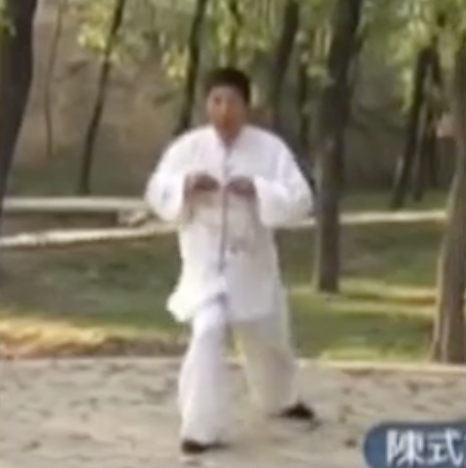
\includegraphics[width=1cm, height=1cm]{images/intro_image/Driving_5.png} &
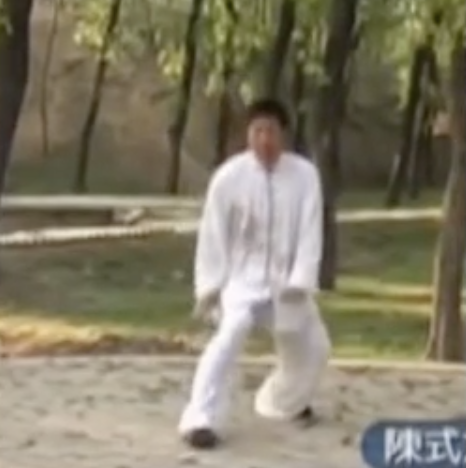
\includegraphics[width=1cm, height=1cm]{images/intro_image/Driving_6.png}\\
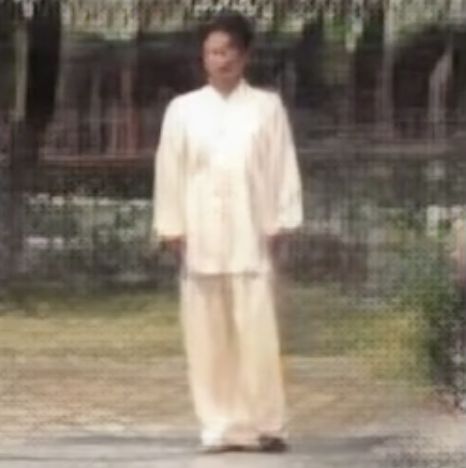
\includegraphics[width=1cm, height=1cm]{images/intro_image/animate_1.png} &
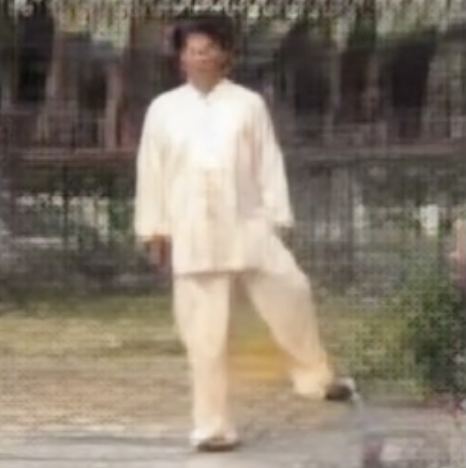
\includegraphics[width=1cm, height=1cm]{images/intro_image/animate_2.png} &
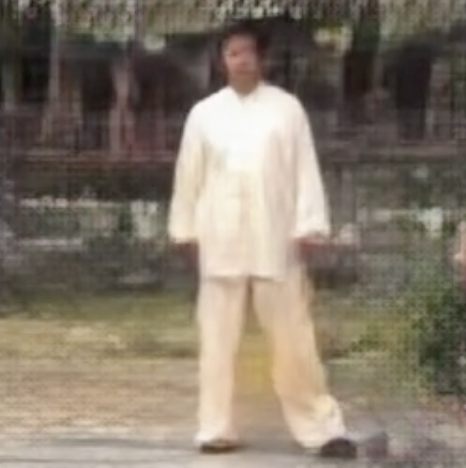
\includegraphics[width=1cm, height=1cm]{images/intro_image/animate_3.png} &
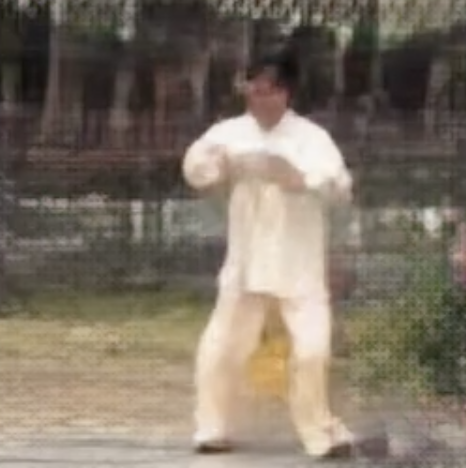
\includegraphics[width=1cm, height=1cm]{images/intro_image/animate_4.png} &
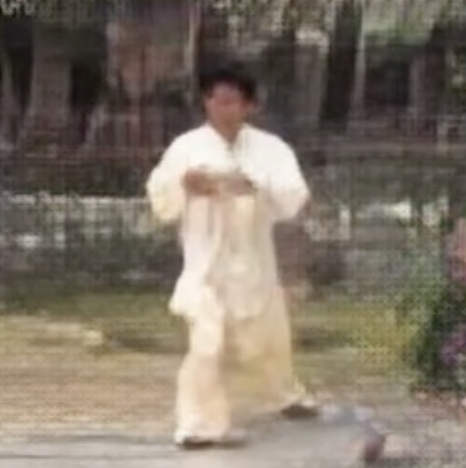
\includegraphics[width=1cm, height=1cm]{images/intro_image/animate_5.png} &
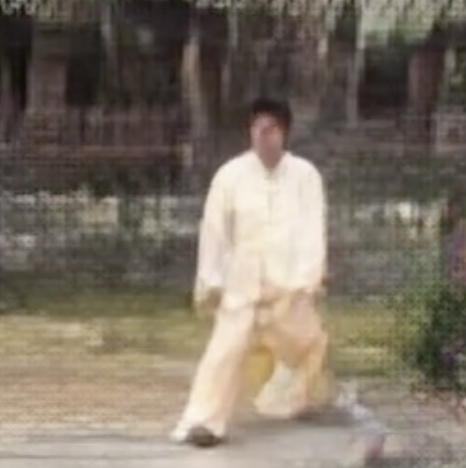
\includegraphics[width=1cm, height=1cm]{images/intro_image/animate_6.png}\\
\bottomrule
\end{tabular}
\end{sc}
\end{small}
\end{center}
\vskip -0.1in
\end{table}

\begin{abstract}
Motion transfer is the task of synthesizing future video frames of a single
source image according to the motion from a given driving video.
This task is challenging due to the complexity of motion representation
and the unknown relations between the driving video and the source image.
Despite this difficulty, this problem attracted great interests from
researches at the recent years, with gradual improvements. The
problem can be thought as decoupling of motion and appearance, which is
often solved by extracting the motion from keypoint movement.
We chose to tackle the generic, unsupervised setting, where we need to apply
animation to any arbitrary object, without any domain specific model for the
structure of the input.
In this work, we extract the structure from a keypoint heatmap, without an
explicit motion representation. Then, the structures from the image and the
video are extracted to warp the image according to the video, by a deep
generator.
\end{abstract}

\section{Introduction}
Take a look at Figure ~\ref{table:intro} for two video sequences. The input
is a YouTube clip of a Thai-Chi artist (the driving subject) performing a
series of complex motions in the top row. Our algorithm's output is shown in
the bottom row. It refers to frames that appear to show a different person
(the source subject) executing the same motions. The twist is that the
source individual has never performed the same exact sequence of motions as
the driver video. In reality, he was photographed doing another movement
with no clear reference to the driving's actions.
And, as the figure shows, the source and the driving are of different
appearances, have different backgrounds, and are dressed differently.

In this study, we propose a simple, however surprisingly efficient approach
to the general motion transfer problem, which can be
applied to any domain, similarly to \cite{siarohin2019animating}:
Given a source image of a person with the wanted appearance,
and a driving video with the wanted structure/geometry,
we synthesize a video by applying a deep motion generator per-frame. We
assist the generator by feeding it with compact structural representations
of the source and each frame of the driving video. That way, we obtain the
target of a video of the source appearance and the driving motion, given
any domain.

Researchers of some notable works (Section~\ref{related}) observe that
keypoint-based pose preserves motion signatures over time, while
abstracting subject identities. We therefore use the keypoint-based pattern
without any other motion priors. We obtain the keypoints and use them to
animate images in a way that doesn't need any external information about the
subject or any assumption or prior about the scene.

Our contribution is twofold: first, we demonstrate that removing the motion
prior will function and provide better accuracy outcomes, and second,
we provide a compact representation with improved efficiency.

\medskip

\section{Related Work:}
\label{related}
Motion transfer has gained a lot of coverage over the last twenty years.
Early approaches based on manipulating existing video footage to generate
new content. These included searching for frames in which the body position
corresponds to a desired motion and using them to generate a new
content \cite{bregler1997video}. Our approach is equally designed for videos,
but rather than manipulating existing images, we learn to synthesize new
movements that were never seen before with the new identities.

A number of techniques are based on calibrated multi camera systems to scan
a target player and use an adapted 3D model of the target to control their
motion in a new frame\cite{cheung2004markerless}. Our solution instead
examines the transition of movement between 2D video subjects and prevents
data calibration or 3D space information.

Latest approaches concentrate on the disentangling of appearance and
activity and synthesizing of new motion videos \cite{tulyakov2018mocogan}.
Similarly, we apply our representation of motion to different target
subjects to generate new motions. However, In contrast to these works,
we did not use GAN but an encoder-decoder approach.

In comparison to the pixel-based approaches for image animation that were
common until recently, keypoint-based approaches are now thought to have
the ability to achieve high performance in the field of video reanimation.
Some notable works in
this area are \cite{siarohin2020order},
\cite{siarohin2019animating}, \cite{kim2019unsupervised},
\cite{balakrishnan2018synthesizing}, \cite{ma2017pose},
\cite{reed2017parallel}, \cite{chan2019everybody}.


Our work does not depend on a strong
motion prior directly, but rather on a
structure mask derived from a keypoint detector of a motion-based model,
such as \cite{siarohin2020order}. The idea of using drawn keypoints as a
geometry representation (structural mask) was already used in image-to-image
translation works such as TransGaGa \cite{wu2019transgaga}, in addition to
some of the video reanimation works mentioned earlier.

The concept of using a structural mask in the context of image animation is
demonstrated in \cite{shalev2020image}. However, the current work differs
by basing the mask off a motion related keypoint module, which saves us the hassle
of perturbing the input hoping to achieve an identity-less mask which might
not even be optimal. That way, we
can base more of the motion representation on the deep network, reduce our
prior, and leave some space for our network to optimize more. We also
purpose an heatmap mask, which differs from some of the drawn keypoint
masks mentioned.

\section{Methodology}
The network can be divided into two parts: obtaining the mask, and generating
the synthesized frame. The generator architecture is constant amongst all of
our variations, and can be described as low resolution generation from the
source image, source mask and driving mask; Followed by up-scaling of the
low scale synthesized prediction by passing it with the source frame to a
high resolution generator.
We created two different versions for the mask generator: the first, an
absolute motion transfer; the second,  a relative motion transfer. We chose
to present the results for the first, absolute one, due to its performance.
The performance drop for our second, relative version was expected because the
mask contained less structural information.
The first version is referred as a "keypoint heatmap," while the second is referred as a "circles mask" or "keypoints after softmax".

\subsection{First mask version for absolute motion transfer, with warping}
Our main mask for the project is obtained from carefully observing the
keypoint module from \cite{siarohin2020order}. U-Net based keypoint
modules of this form, work by extracting features, which pass through a
$\textit{conv}$ layer to form a heatmap image $K$ channels, where $K$ is the
number of keypoints. Then, a softmax is performed over the channels, and
keypoints are extracted from the mean location of each heatmap channel.
By carefully debugging the code, and the expectation for a segmentation map
out of U-Net, we obtain Figure~\ref{mask-10kp}.
\begin{figure}[ht]
\vskip 0.2in
\begin{center}
\centerline{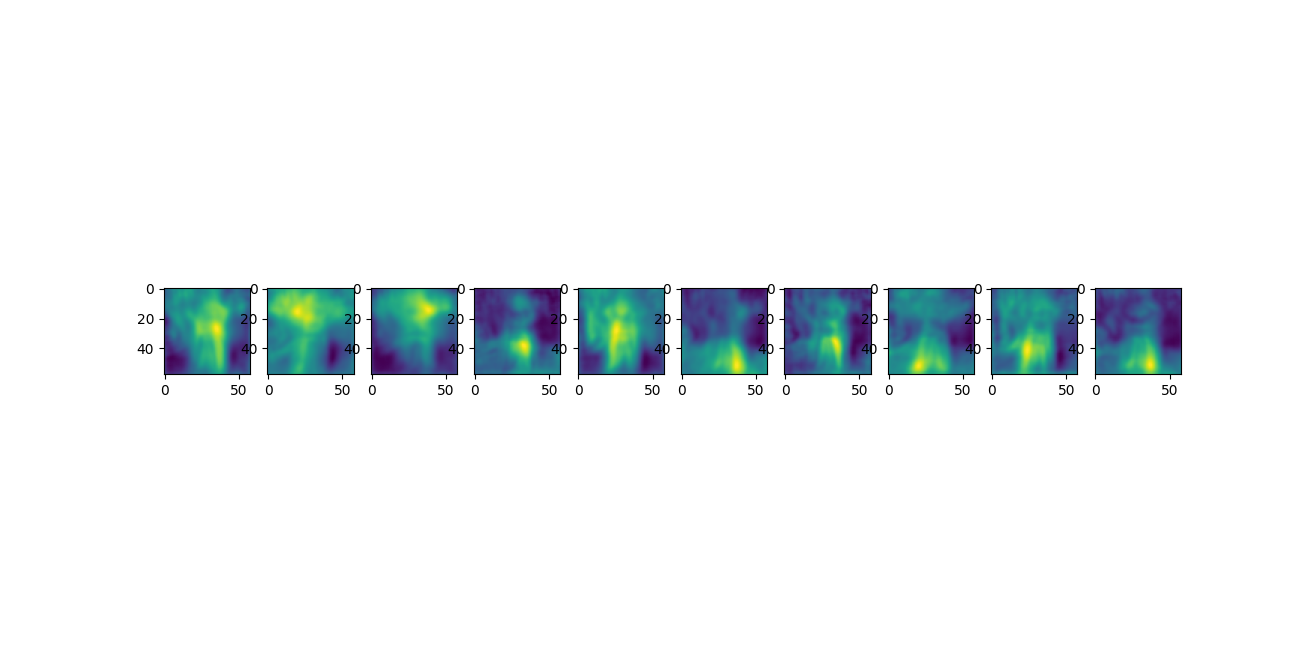
\includegraphics[width=\columnwidth]{visualizations/mask_10kp}}
\caption{
$K$ channels of the keypoint detector network used in
\cite{siarohin2020order}, before the softmax activation. Our main motion
prior in this project.
}
\label{mask-10kp}
\end{center}
\vskip -0.2in
\end{figure}

Summing over the channels, we get Figure~\ref{mask-sum}.

\begin{figure}[ht]
\vskip 0.2in
\begin{center}
\centerline{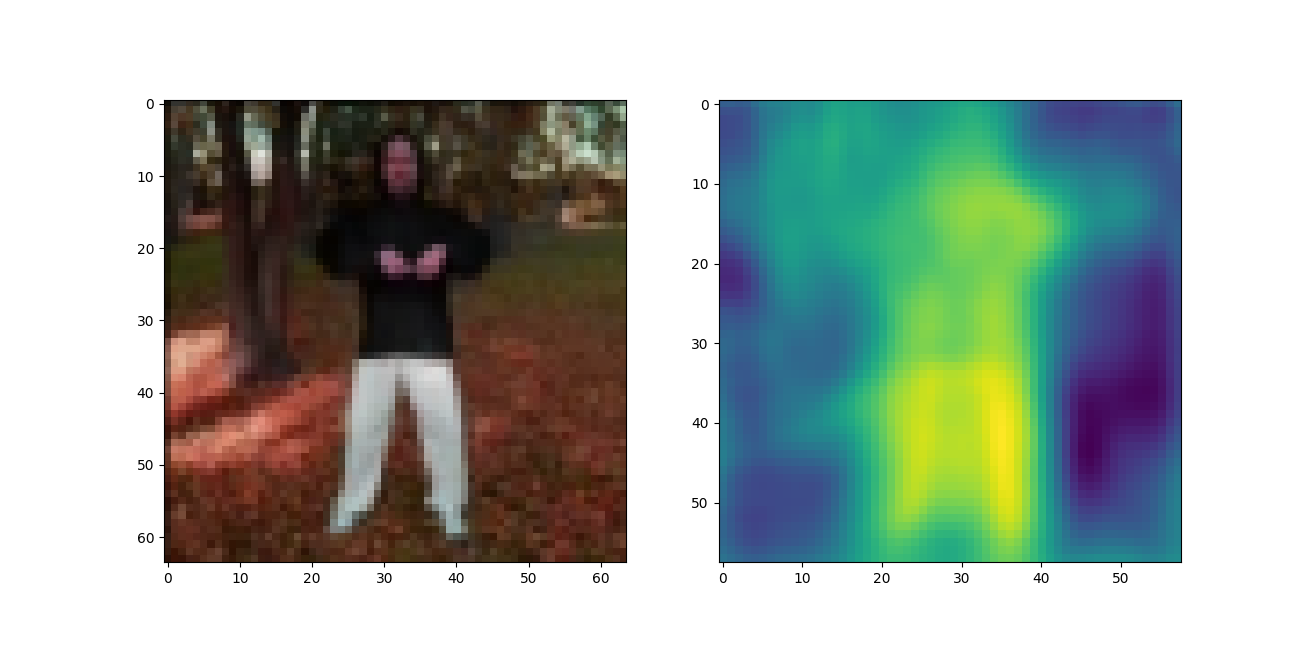
\includegraphics[width=\columnwidth]{visualizations/mask_sum}}
\caption{
The sum of the $K$ channels which is fed as a structural mask into the
generator.
}
\label{mask-sum}
\end{center}
\vskip -0.2in
\end{figure}
which is our output mask, aka the heatmap, pre softmax mask.

\subsection{Second mask version for relative motion transfer}
We purposes an additional "circles" only mask
which can be used in the context
of relative motion transfer during animation, as in
\cite{siarohin2020order}, which isn't possible with the previous heatmap mask.
The mask captures the image's geometry representation \cite{wu2019transgaga},
and by requiring it to be represented as keypoints with a center, we can use
the relative coordinates for the animation. This module, though, did not do
as well as our heatmap mask module (Table~\ref{table:results}).

While relative motion transition is not always desired, this work shows that
a keypoint-only-prior-based module is feasible for the task.
Since the only information contained in the pair of masks is the keypoint
displacement, our deep network can only attempt to approximate a zero order
approximation, we can anticipate results that are more close to
\cite{siarohin2019animating}.

By taking the softmax over the heatmap, we get Table~\ref{softmax-10kp}.
\begin{figure}[ht]
\vskip 0.2in
\begin{center}
\centerline{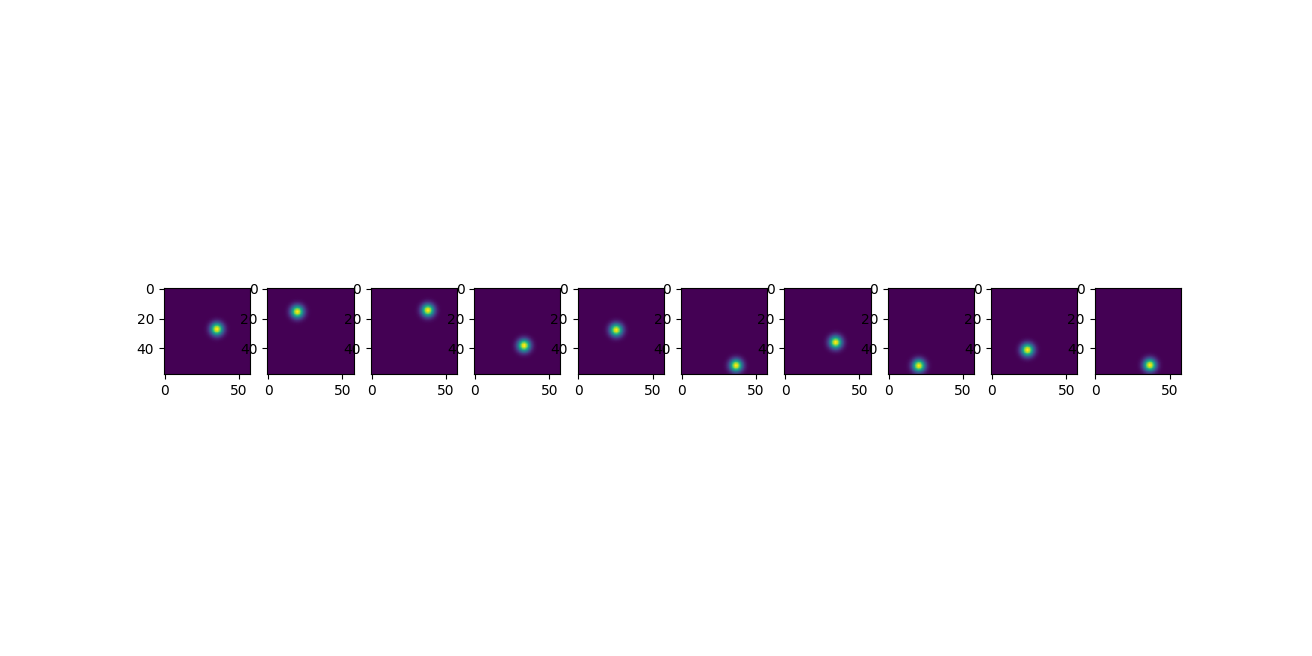
\includegraphics[width=\columnwidth]{visualizations/softmax_10kp}}
\caption{
$K$ channels of the keypoint detector network used in
\cite{siarohin2020order}, after the softmax activation and Gaussian fit.
}
\label{softmax-10kp}
\end{center}
\vskip -0.2in
\end{figure}

Summing over the channels, we get Table~\ref{softmax-sum}.

\begin{figure}[ht]
\vskip 0.2in
\begin{center}
\centerline{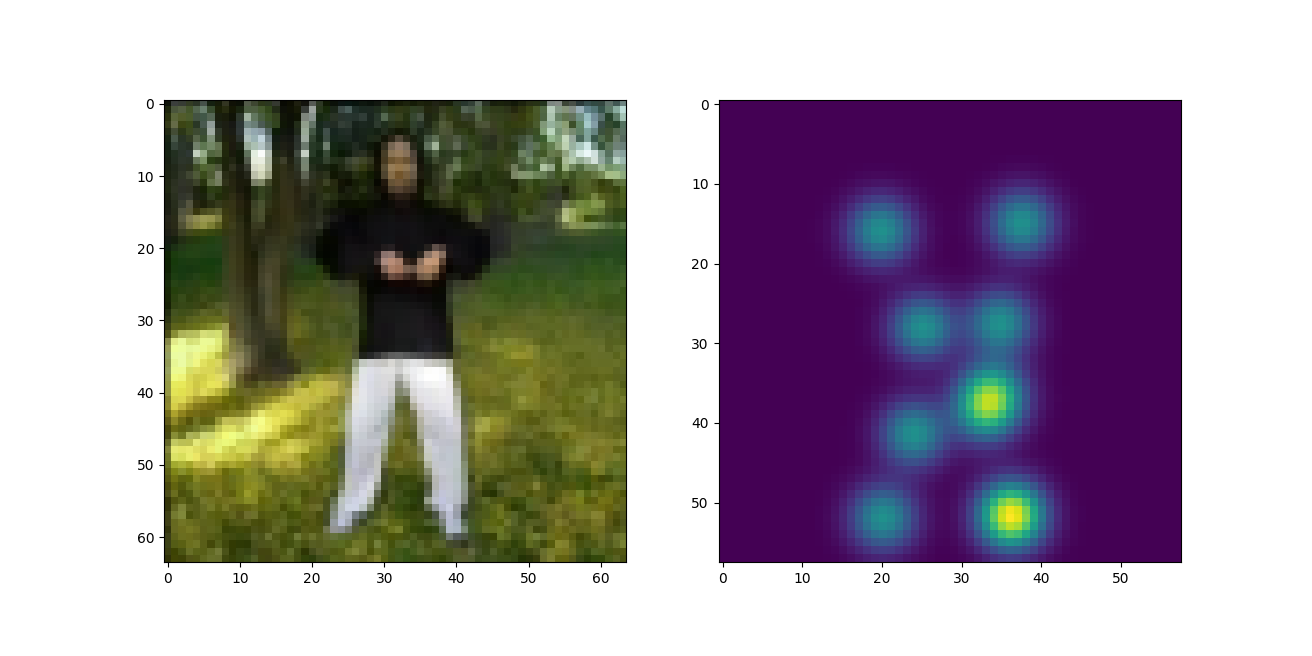
\includegraphics[width=\columnwidth]{visualizations/softmax_sumkp}}
\caption{
The sum of the $K$ channels which is fed as a structural mask into the
generator.
}
\label{softmax-sum}
\end{center}
\vskip -0.2in
\end{figure}
which is our output mask, aka the keypoints after softmax mask.

\subsection{Architecture}
\label{method}

\begin{figure}[ht]
\vskip 0.2in
\begin{center}
\centerline{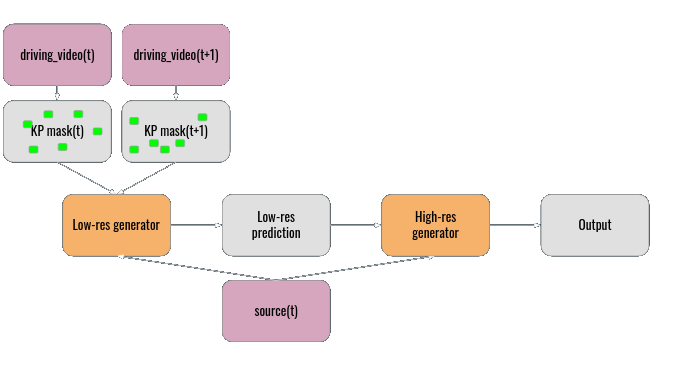
\includegraphics[width=\columnwidth]{visualizations/architecture}}
\caption{Architecture of the model. The keypoint mask can be either a
keypoint heatmap such as in Figure~\ref{mask-sum}, or drawn keypoint
circles as in Figure~\ref{softmax-sum}.}
\label{arch}
\end{center}
\vskip -0.2in
\end{figure}

Our architecture follows \cite{siarohin2020order} without the dense
motion module, after changing its keypoint generation module to return our
mask. After the mask is obtained, we follow the encoder decoder approach as
\cite{shalev2020image}.
Namely, the encoder of the low resolution generator consists of $\textit{conv}_{7
\times 7}$, $\textit{batch\_norm}$, $\textit{relu}$, followed by six
residual blocks of $\textit{batch\_norm}$, $\textit{relu}$,
$\textit{conv}_{3 \times 3}$ ,$\textit{batch\_norm}$, $\textit{relu}$,
$\textit{conv}_{3 \times 3}$, (and a sum with the source).
The residual blocks help to maintain the identity of the source image
\cite{he2015deep}.
The decoder consists of two blocks, each is a sequence of
$\textit{up\_sample}_{2 \times 2 }$, $\textit{batch\_norm}$,
$\textit{relu}$. The decoder is followed by a $\textit{conv}_{7 \times 7}$
and a $\textit{sigmoid}$ activation.
For the high resolution generator, use an encoder (decoder) with five encoding (decoding) blocks,
where each block is a sequence of
$\textit{conv}_{3 \times 3}$, $\textit{batch\_norm}$, $\textit{relu}$
$\textit{avg\_pool}_{2 \times 2}$, and each decoding block is a sequence of
$\textit{up\_sample}_{2 \times 2}$, $\textit{conv}_{3 \times 3}$,
$\textit{batch\_norm}$, $\textit{relu}$.
We add skip connections from each of the encoding layers to its
corresponding encoding layer, to form a U-Net architecture
\cite{ronneberger2015unet}.


\subsection{Losses}
We use the same perceptual loss as in \cite{siarohin2020order} which is
based on the implementation of \cite{wang2018videotovideo}. With the input
driving frame $D$ and the corresponding reconstructed frame $\hat{D}$, the
reconstruction loss is written as: $L_{rec}(\hat{D}, D) =
\sum_{i=1}^{I} |N_i(\hat{D})-N_i(D)|$, where $N_i(\cdot)$ is the $i^{th}$
channel feature extracted from a specific VGG-19 layer \cite{simonyan2015deep}
and $I$ is the number of feature channels in this layer. Additionally we use this lose on
a number of resolutions, forming a pyramid obtained by down-sampling
$\hat{D}$ and $D$, similarly to \cite{}, \cite{}. The resolutions are $256
\times 256$, $128 \times 128$, $64 \times 64$ and $32 \times 32$.


\section{Experiments}
\subsection{Datasets}
The Tai-chi-HD dataset, which includes brief videos of people doing Tai-chi
exercises, was used for training and evaluation. Following
\cite{siarohin2020order}, 3,141 Tai-chi videos were downloaded from YouTube.
The videos were cropped and resized to a resolution of $256^2$, while the
aspect ratio was preserved. There are 3,016 training videos and 125
evaluation videos.

\begin{table}[t]
\caption{Images comparison}
\label{table:images}
\vskip 0.15in
\begin{center}
\begin{small}
\begin{sc}
\begin{tabular}{m{1.0cm}m{1.0cm}m{1.0cm}m{1.0cm}m{1.0cm}m{1.0cm}}
\toprule
Source image & Driving\\
\toprule
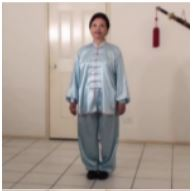
\includegraphics[width=1cm, height=1cm]{images/source} &
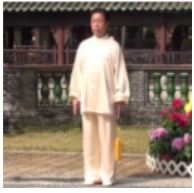
\includegraphics[width=1cm, height=1cm]{images/driving_1} &
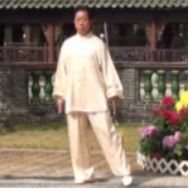
\includegraphics[width=1cm, height=1cm]{images/driving_2} &
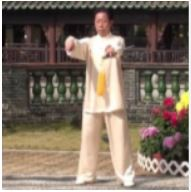
\includegraphics[width=1cm, height=1cm]{images/driving_3} &
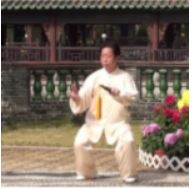
\includegraphics[width=1cm, height=1cm]{images/driving_4} &
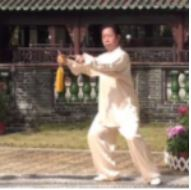
\includegraphics[width=1cm, height=1cm]{images/driving_5} \\
\midrule
X2Face & 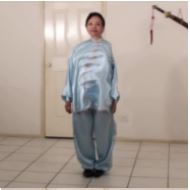
\includegraphics[width=1cm, height=1cm]{images/1_X2Face_1} &
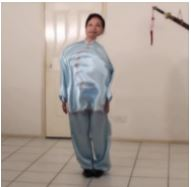
\includegraphics[width=1cm, height=1cm]{images/1_X2Face_2} &
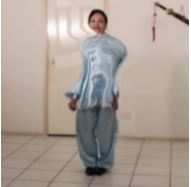
\includegraphics[width=1cm, height=1cm]{images/1_X2Face_3} &
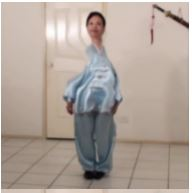
\includegraphics[width=1cm, height=1cm]{images/1_X2Face_4} &
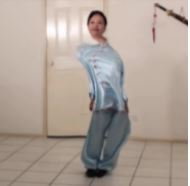
\includegraphics[width=1cm, height=1cm]{images/1_X2Face_5} \\
Monkey-Net & 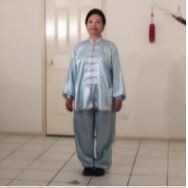
\includegraphics[width=1cm, height=1cm]{images/2_Monkey-Net_1} &
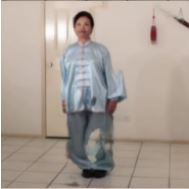
\includegraphics[width=1cm, height=1cm]{images/2_Monkey-Net_2} &
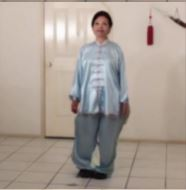
\includegraphics[width=1cm, height=1cm]{images/2_Monkey-Net_3} &
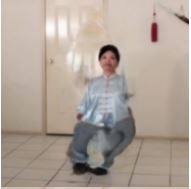
\includegraphics[width=1cm, height=1cm]{images/2_Monkey-Net_4} &
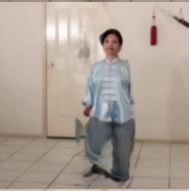
\includegraphics[width=1cm, height=1cm]{images/2_Monkey-Net_5} \\
FOMM & 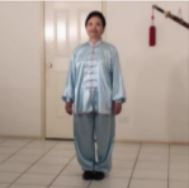
\includegraphics[width=1cm, height=1cm]{images/3_FOMM_1} &
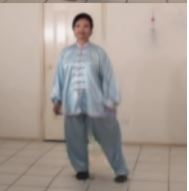
\includegraphics[width=1cm, height=1cm]{images/3_FOMM_2} &
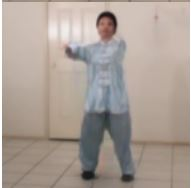
\includegraphics[width=1cm, height=1cm]{images/3_FOMM_3} &
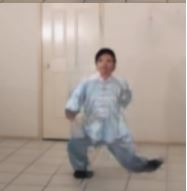
\includegraphics[width=1cm, height=1cm]{images/3_FOMM_4} &
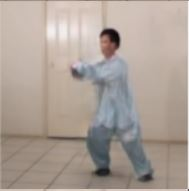
\includegraphics[width=1cm, height=1cm]{images/3_FOMM_5} \\
Perturbed Mask & 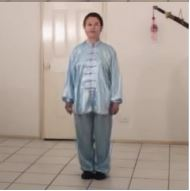
\includegraphics[width=1cm,
height=1cm]{images/4_Perturbed_1} &
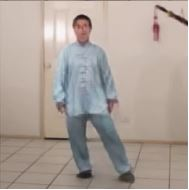
\includegraphics[width=1cm, height=1cm]{images/4_Perturbed_2} &
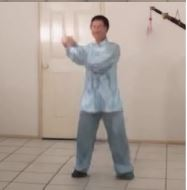
\includegraphics[width=1cm, height=1cm]{images/4_Perturbed_3} &
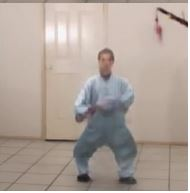
\includegraphics[width=1cm, height=1cm]{images/4_Perturbed_4} &
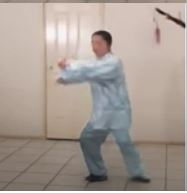
\includegraphics[width=1cm, height=1cm]{images/4_Perturbed_5} \\
Ours & 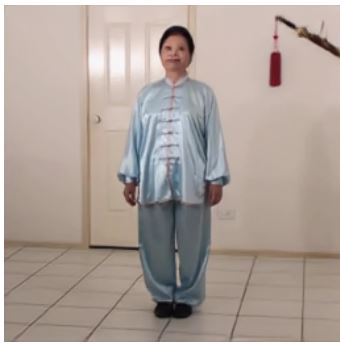
\includegraphics[width=1cm, height=1cm]{images/5_Ours_1} &
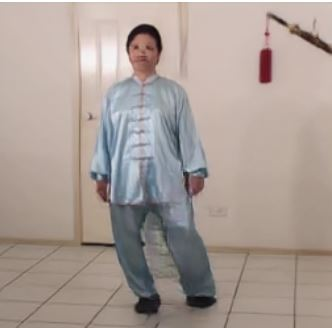
\includegraphics[width=1cm, height=1cm]{images/5_Ours_2} &
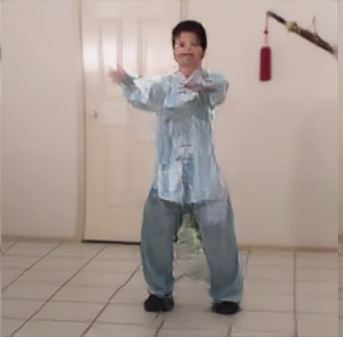
\includegraphics[width=1cm, height=1cm]{images/5_Ours_3} &
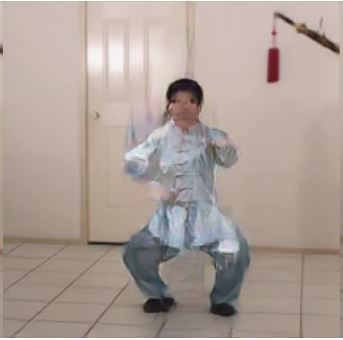
\includegraphics[width=1cm, height=1cm]{images/5_Ours_4} &
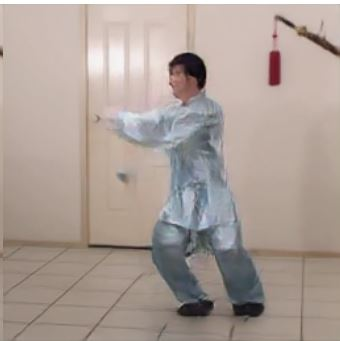
\includegraphics[width=1cm, height=1cm]{images/5_Ours_5} \\
\bottomrule
\end{tabular}
\end{sc}
\end{small}
\end{center}
\vskip -0.1in
\end{table}


\begin{table}[t]
\caption{Images comparison 2}
\label{table:images 2}
\vskip 0.15in
\begin{center}
\begin{small}
\begin{sc}
\begin{tabular}{m{1.0cm}m{1.0cm}m{1.0cm}m{1.0cm}m{1.0cm}m{1.0cm}}
\toprule
Source image & Driving\\
\toprule
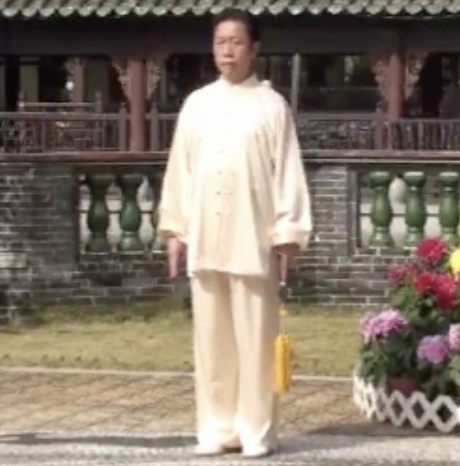
\includegraphics[width=1cm, height=1cm]{images/intro_image/source.png} &
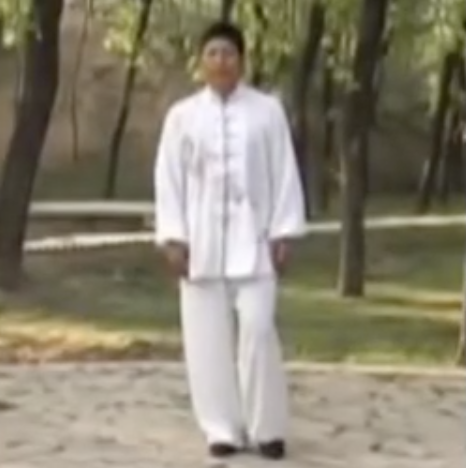
\includegraphics[width=1cm, height=1cm]{images/intro_image/Driving_1.png} &
\includegraphics[width=1cm, height=1cm]{images/intro_image/Driving_2.png} &
\includegraphics[width=1cm, height=1cm]{images/intro_image/Driving_4.png} &
\includegraphics[width=1cm, height=1cm]{images/intro_image/Driving_5.png} &
\includegraphics[width=1cm, height=1cm]{images/intro_image/Driving_6.png} \\
\midrule
FOMM & \includegraphics[width=1cm, height=1cm]{images/intro_image/animate_1_fomm.png} &
\includegraphics[width=1cm, height=1cm]{images/intro_image/animate_2_fomm.png} &
\includegraphics[width=1cm, height=1cm]{images/intro_image/animate_4_fomm.png} &
\includegraphics[width=1cm, height=1cm]{images/intro_image/animate_5_fomm.png} &
\includegraphics[width=1cm, height=1cm]{images/intro_image/animate_6_fomm.png} \\
Ours & \includegraphics[width=1cm, height=1cm]{images/intro_image/animate_1.png} &
\includegraphics[width=1cm, height=1cm]{images/intro_image/animate_2.png} &
\includegraphics[width=1cm, height=1cm]{images/intro_image/animate_4.png} &
\includegraphics[width=1cm, height=1cm]{images/intro_image/animate_5.png} &
\includegraphics[width=1cm, height=1cm]{images/intro_image/animate_6.png} \\
Ours (softmax)&
\includegraphics[width=1cm, height=1cm]{images/softmax/01.png} &
\includegraphics[width=1cm, height=1cm]{images/softmax/02.png} &
\includegraphics[width=1cm, height=1cm]{images/softmax/04.png} &
\includegraphics[width=1cm, height=1cm]{images/softmax/05.png} &
\includegraphics[width=1cm, height=1cm]{images/softmax/06.png} \\
\bottomrule
\end{tabular}
\end{sc}
\end{small}
\end{center}
\vskip -0.1in
\end{table}

\subsection{Comparison with Previous Works}
In order to compare our work to previous works (Table~\ref{table:results})
we used metrics previously used in similar papers.
Average Key-points Distance \cite{cao2017realtime} (AKD)
measures the average key-points distance between the generated video and
the source video. Average Euclidean Distance \cite{zheng2019joint} (AED)
measures the average euclidean distance
 between the representations of the ground-truth and generated videos in
 some embedding space. In addition, we added the L1 distance as well.
 Our AED and AKD metrics were calculated using the following repository:
 \url{https://github.com/AliaksandrSiarohin/pose-evaluation}
\\
Note that those metrics aren't optimal since one can easily improve
reconstruction by increasing the bottleneck, and we can see our
artifacts in animation results (Table~\ref{table:images}).
However, our pose did follow the driving video well, and to improve the
identity and background artifacts, we suggest some fixes in Section~\ref{future}.

% Note use of \abovespace and \belowspace to get reasonable spacing
% above and below tabular lines.

\begin{table}[t]
\caption{Accuracy Metrics}
\label{table:results}
\vskip 0.15in
\begin{center}
\begin{small}
\begin{sc}
\begin{tabular}{lcccr}
\toprule
Method & AKD & AED & L1 \\
\midrule
X2Face    & 17.654 & 0.272 & 0.080 \\
Monkey-Net    & 10.798 & 0.228 & 0.077 \\
FOMM    & 6.872 & 0.167 & 0.063 \\
Perturbed Mask & 4.239 & 0.147 & 0.047 \\
Ours (circles mask) & 14.760& 0.245 & 0.077 \\
Ours & 5.551 & 0.141 &  0.045\\
\midrule
Improvement (FOMM)    & 19.2\% & 15.5\% & 28.5\% \\
\bottomrule
\end{tabular}
\end{sc}
\end{small}
\end{center}
\vskip -0.1in
\end{table}
\section{Future work}
\label{future}
We would like to test our module on more datasets, and compare them to the
state of the art. In addition, summing the heatmap channels might not be
optimal, and there is certainly some space to try something deeper with the
features extracted in the keypoint detector as an input, or feed all of the
channels separately into the generator. We want to experiment with
mask thresholds due to the distortions in the animation background.
We may also increase the number of keypoints, but that would probably be
more beneficent to the second type of mask, and would increase the
required GPU memory proportionally. We also thought about coloring
matching keypoints with the same color to help the module to learn a motion
flow.

\section{Conclusions}
We constructed a novel method for image animation by moving the need for
a strong motion prior (optical flow) to the assumption of a pre-trained
keypoint detector/keypoint heatmaps prior to activation, which might be
based on a motion prior.
By doing so, we encapsulated motion to a motion mask, which is
bottlenecked by the prior training which has the keypoint bottleneck.
The motion masks are then fed into a generator, which combines the
appearance of the source image and the mask which represents the structure,
decoupled from any appearance naturally by the assumption that during the
training of the keypoint detector, the heatmap mask went into a keypoint
bottleneck. After evaluation, we can conclude that our method is
feasible, although with some artifacts.
\section*{Software and Data}
Detailed in our repository:
\\
\url{https://github.com/or-toledano/
animation-with-keypoint-mask}
\bibliography{animation-with-keypoint-mask}
\bibliographystyle{icml2021}

\end{document}
